\chapter{Photon-Ring Substructure}
\label{ch:ring}

\section{Sub-ring decomposition by crossing count}
\label{sec:subrings}

Binning image pixels by the number of prior equatorial crossings isolates
the photon sub-rings \citep{Johnson2020}: the direct image ($n=0$), the
first lensed ring ($n=1$), and the second ring ($n=2$)
(\texttt{SubRingExtractor::analyze} in
\texttt{science/photon\_ring/}). The bolometric
flux ratios are $F_0/F_1 = \FluxRatioZeroOne$ and
$F_1/F_2 = \FluxRatioOneTwo$ (Fig.~\ref{fig:subrings}), the steep
$n=1 \to n=2$ demagnification reflecting the exponential suppression
$e^{-\gamma}$ per half-orbit near the critical curve, with $\gamma$ the
Lyapunov exponent of the bound photon orbits. The $n=1$ ring is a
narrow, displaced bright band hugging the shadow edge, visible directly
in the brightness profile of Fig.~\ref{fig:profile}; its measured radial
width at this geometry is a few per cent of the shadow diameter
(\texttt{scan\_widths}), qualitatively the regime in which
\citet{Johnson2020} project that space--ground interferometry could detect
the $n=1$ signature in the visibility-domain power-law tail. Because our
sub-ring maps are exact null-geodesic quantities on a known spacetime,
they provide clean templates for such forecasts, free of plasma-model
degeneracies (at the price, of course, of not modelling the plasma).

\begin{figure}
\centering
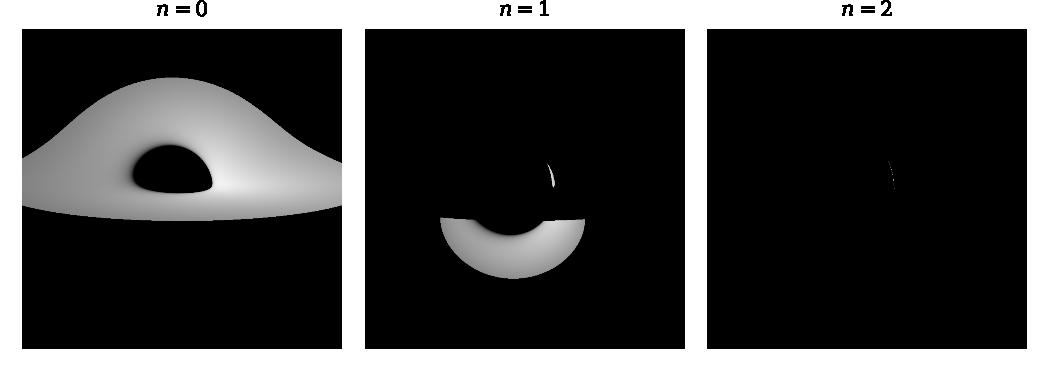
\includegraphics[width=\textwidth]{figures/fig_subrings.pdf}
\caption{Bolometric maps of the photon sub-rings $n=0,1,2$ (log stretch).
Flux ratios: $F_0/F_1=\FluxRatioZeroOne$, $F_1/F_2=\FluxRatioOneTwo$.}
\label{fig:subrings}
\end{figure}

\begin{figure}
\centering
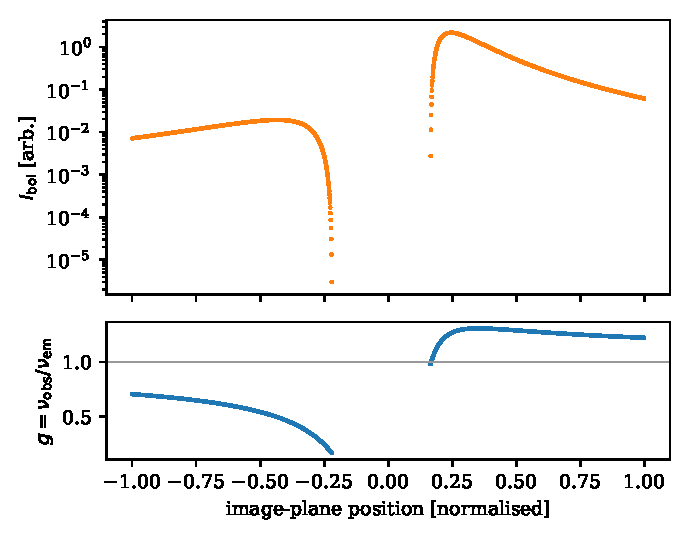
\includegraphics[width=0.62\textwidth]{figures/fig_brightness_profile.pdf}
\caption{Bolometric intensity along the image major axis. The narrow
$n=1$ sub-ring stands on the shoulder of the direct disk image at the
shadow edge.}
\label{fig:profile}
\end{figure}

\section{Sub-ring metrics across the spin range}
\label{sec:subringsweep}

\stub{Sub-ring flux ratio and width vs $\astar$ (needs the
\texttt{subring\_tool --sweep} extension); the Johnson et al.\ universal
parameters; connection to the Lyapunov exponents of
Chapter~\ref{ch:shadow}.}

\section{The axial image tower}
\label{sec:axialtower}

\stub{User-requested topic (THESIS\_PLAN Part 1c): the bright vertical
columns along the spin axis seen in near-edge-on renders are the
gravitationally-lensed polar caustic --- stacked higher-order images of the
far/underside of the disk funnelled along the axis --- NOT an
astrophysical jet. Contrast with real relativistic jets
(Blandford--Znajek, MHD-driven), which require plasma physics outside this
thin-disk + geodesic model. Awaiting the user's engine render; the caption
will carry the exact \texttt{sgr\_engine} reproduction command.}

\section{Detectability forecast}
\label{sec:ngeht}

\stub{ngEHT-class detectability of the $n=1$ signature; visibility-domain
power-law tail; what the exact-geodesic templates provide.}
